\documentclass[12pt]{article}

% Set page size and margins
\usepackage[letterpaper,top=2cm,bottom=2cm,left=3cm,right=3cm,marginparwidth=1.75cm]{geometry}

% Useful packages
\usepackage{graphicx}
\usepackage{amsmath}

\title{AM 213A HW3}
\author{Joseph Moore}
\date{Winter 2022}

\newenvironment{amatrix}[1]{%
	\begin{array}{@{}*{#1}{c}|c@{}}
	}{%
	\end{array}
}

\begin{document}

\maketitle

\title{\textbf{Part 1}}


\paragraph{1.}
	\subparagraph{$\bullet$}
		We can show that a positive definite matrix can be written as lower triangular matrix multiplied by its conjugate transpose. We end up with the equations 2.82 and 2.83. We've seen before how $Ax = b$ can easily be solves with substitution if $A$ is triangular. Using this fact we have
    	\[
    	A^TAx = A^Tb = \tilde{A}x = \tilde{b} = LL^*x = \tilde{b}.
    	\] 
    	Then we solve $Ly = \tilde{b}$ for $y$ and then $L^*x = y$ for $x$ which is the solution to our original equation.
    
    \subparagraph{$\bullet$}
    	The resulting equation for the third degree polynomial fit is 
    	\[
    	f(x) = 1.83 - 5.17x + 11.2x^2 - 7.28x^3.
    	\]
    	The 2-norm of the resulting error $E = ||b - Ax|| = 6.98\cdot10^{-6}$. Below is the resulting fitted curve.
    	
    	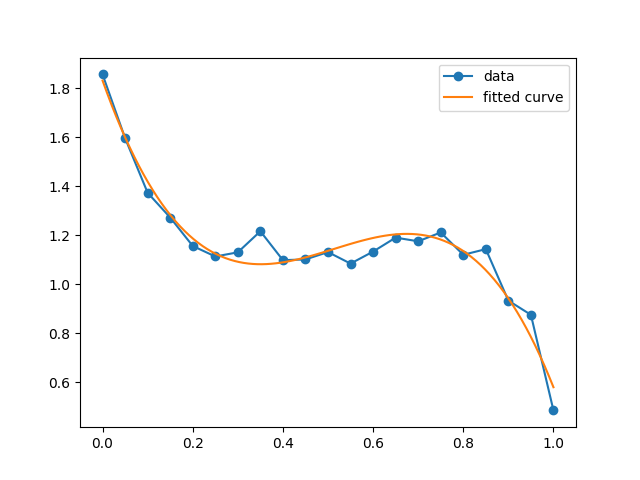
\includegraphics[scale=0.7]{Figure_1}
    	
    \subparagraph{$\bullet$}
    	The resulting equation for the fifth degree polynomial fit is 
    	\[
    	f(x) = 1.87 - 7.25x + 28.8x^2 - 58.7x^3 + 61.0x^4 - 25.2x^5.
    	\]
    	The 2-norm of the resulting error $E = ||b - Ax|| = 2.84\cdot10^{-5}$. Below is the resulting fitted curve.
    	
    	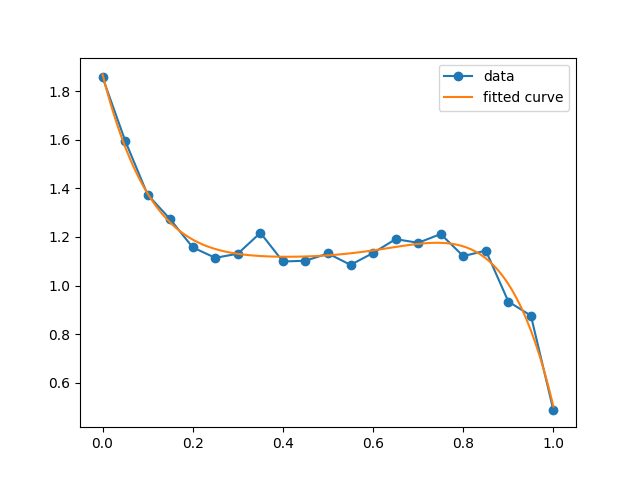
\includegraphics[scale=0.7]{Figure_2}
    	
    \subparagraph{$\bullet$}
    	single precision floats only store numbers from $10^{-38}$ up to $10^{38}$. When values carry essential information up to the sixth significant digit then being raised to anything over the fifth power will result in a lose of information. 
    	
    	From my code I found that fitting a curve up to the sixth degree polynomial resulted in significant error. 
    	
    
\paragraph{2.}
	\subparagraph{$\bullet$}
		\[
		H_jA = A - 2v_jv_j^TA = A - 2
		\left(\begin{matrix}
		0 \\
		0 \\
		a_{jj} + s_j \\
		: \\
		a_{mj} \\
		\end{matrix}\right)
		\left(\begin{matrix}
		0 & 0 & a_{jj} + s_j & ... & a_{mj}
		\end{matrix}\right)
		A
		\]\[
		= A - 2
		\left(\begin{matrix}
		0 & 0 & 0 & 0 & 0 & 0\\
		0 & 0 & 0 & 0 & 0 & 0\\
		0 & 0 & (a_{jj} + s_j)^2 & ... & ... & (a_{jj} + s_j)a_{mj} \\
		0 & 0 & : & : & : & : \\
		: & : & : & : & : & : \\
		0 & 0 & (a_{jj} + s_j)a_{mj} & ... & ... & a_{mj}^2 \\
		\end{matrix}\right)
		\left(\begin{matrix}
		a_{11} & a_{12} & ... & a_{1n} \\
		a_{21} & a_{22} & ... & a_{2n} \\
		: & : & : & : \\
		a_{n1} & a_{n2} & ... & a_{nn} \\
		\end{matrix}\right)
		\]
		
		... IDK
		
	\subparagraph{$\bullet$}
		The resulting equation for the third degree polynomial fit is 
		\[
		f(x) = 1.83 - 5.17x + 11.2x^2 - 7.28x^3.
		\]
		The 2-norm of the resulting error $E = ||b - Ax|| = 0.244575$. Below is the resulting fitted curve.
		
		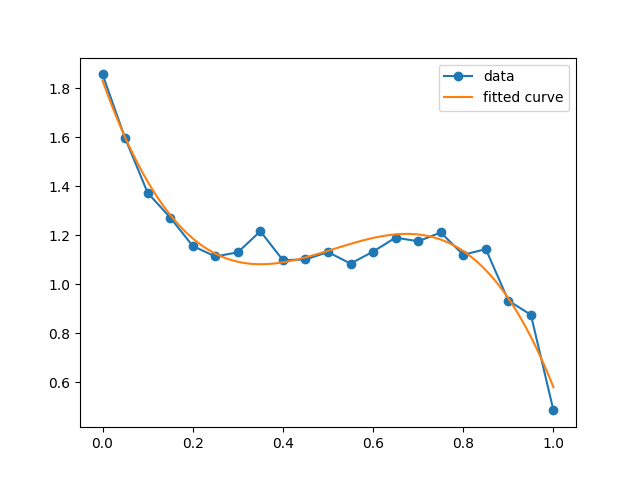
\includegraphics[scale=0.7]{Figure_3}
		
	\subparagraph{$\bullet$}
		The resulting equation for the fifth degree polynomial fit is 
		\[
		f(x) = 1.87 - 7.26x + 28.8x^2 - 58.8x^3 + 61.1x^4 - 25.2x^5.
		\]
		The 2-norm of the resulting error $E = ||b - Ax|| = 2.84\cdot10^{-5}$. Below is the resulting fitted curve.
		
		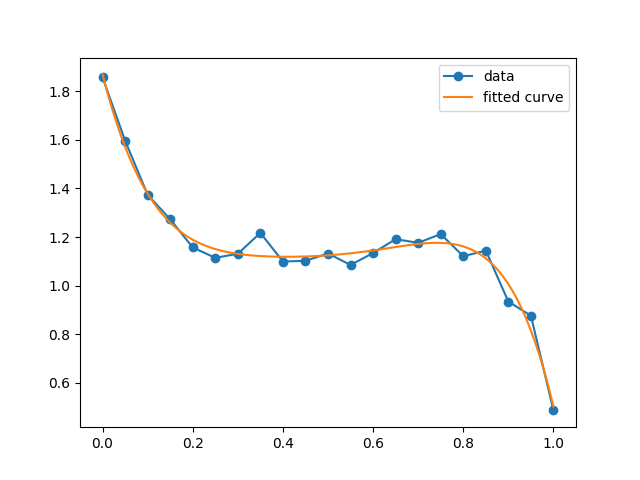
\includegraphics[scale=0.7]{Figure_4}
		
	\subparagraph{$\bullet$}
		The algorithm begins to break down around the 12th polynomial but is fine up until that point. 
		
		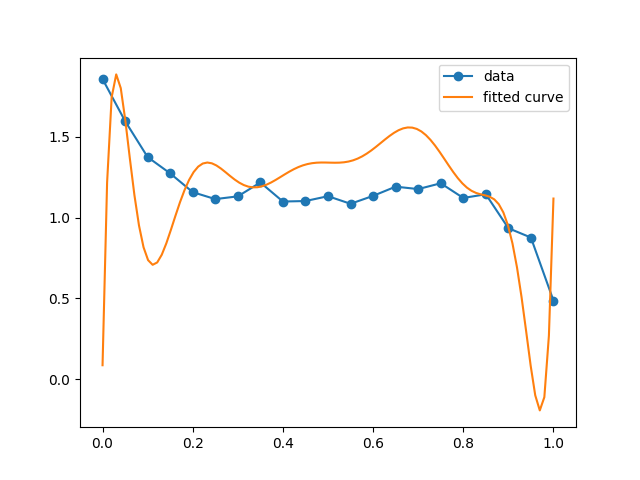
\includegraphics[scale=0.7]{Figure_5}
		
	\subparagraph{$\bullet$}
		We have $||A - QR|| = 2.166\cdot10^{-06}$ and $||Q^T*Q - I|| = 2.658$. This means that the accuracy of our decomposition is high where as the orthogonality of Q is low.
		
		

\newpage	
\title{\textbf{Part 2}}


\paragraph{1.}
	We must show that $(I-2P)^*(I-2P) = (I-2P)(I-2P)^* = (I-2P)(I-2P)^{-1} = I$. We know that $P^* = P^2 = P$ and can then show that
	\[
	(I-2P)^*(I-2P) = (I^*-2P^*)(I-2P) = (I-2P)(I-2P) = I - 2P - 2P + 4P^2 = I - 4P + 4P = I.
	\]
	
\paragraph{2.}
	\subparagraph{a)}
		Using the Cauchy-Schwarz inequality and the fact that $P = P^2$ we can say
		\[
		||P||_2 = ||P^2||_2 \le ||P||^2_2.
		\]
		Divide everything by $||P||_2$ and you get $1 \le ||P||_2$. $P$ being orthogonal means that
		\[
		||Py|| = ||y|| \le ||P||\cdot||y||	
		\]
		Divide everything by $||P||$ and we have
		\[
		\frac{||Py||}{||P||} = \frac{||y||}{||P||} = 1 \le ||y||
		\]
				
\paragraph{3.}
	\subparagraph{a)}
		We can write our matrix as $A = QR$ where $A$ and $Q$ can be written as columns $A = (a_1, a_2, a_3, ...)$ and $Q = (q_1, q_2, q_3, ...)$ and $R$ as standard matrix elements $r_{ij}$. Then 
		\[
		A = (a_1, ... , a_n) = 
		\left(\begin{matrix}
		q_1 & ... & q_n
		\end{matrix}\right)
		\left(\begin{matrix}
		r_{11} & r_{12} & ... & r_{1} \\
		r_{21} & r_{22} & ... & : \\ 
		: & : & : & :\\ 
		r_{n1} & r_{n2} & ... & r_{nn}
		\end{matrix}\right)
		\]
		so that we can write 
		\[
		a_j = \sum_{i=1}^{j}r_{ij}q_i = \sum_{i=1}^{j-1}r_{ij}q_i + r_{jj}q_j
		\]
		and we see that $a_j$ is in the span of the columns of $Q$ up to $q_j$. Likewise, the columns of $A$ up to $a_{j-1}$ are all in the span of $Q$ up to $q_{j-1}$ Remembering that the columns of $Q$ are all linearly independent we can say $a_j$ can only be linearly independent from the previous columns if it has a nonzero contribution from $q_j$. In other words, $a_j$ can only be linearly independent from the previous columns if $r_{jj}$ is non-zero and if $r_{jj}$ is non-zero then $a_j$ must be linearly independent from the previous columns.
		
	\subparagraph{b)}
		Because $r_{jj}$ being non-zero means that $a_j$ is linearly independent from all previous columns then the number of linearly independent columns must be equal to the number of non-zero diagonal elements.
		
\paragraph{4.}
	The projection of a vector x onto a vector v is $(\frac{v^Tx}{v^tv})v$ and thus the projection onto the plane orthogonal to v is simply x minus this component or $x - (\frac{v^Tx}{v^tv})v$. If we want to reflect across this plane we simply subtract the parallel component twice and get $x - 2(\frac{v^Tx}{v^tv})v$ which is the Householder transformation applied to x. This geometric description leads us to see that the transformation hold all dimensions constant except the one parallel to v and that v must be an eigenvector with a corresponding eigenvalue of -1. All other eigenvalues must be 1. 
	
	If x $\perp$ v then Hx = x - $2\frac{v^Tx}{v^Tv}$ = x - 0 = x. Thus x is a eigenvector with corresponding eigenvalue 1. Where as if x $\parallel$ v then Hx = x - 2$\frac{||v||^2x}{||v||^2}$ = x - 2x = -x and thus x is a eigenvector with corresponding eigenvalue of -1. Because H is symmetric we know that the singular values are $|\lambda_i|$ then they must all be 1. Because only one eigenvalue will be 1, the eigenvalue corresponding to the eigenvector orthogonal to the plane of reflection, and all the other eigenvalues will be 1, then the determinant, being the product of all the eigenvalues, will be -1.
	
\paragraph{5.}
	\[
	\kappa(A^TA) = \frac{max_{||x||=1}||A^TAx||}{min_{||x||=1}||A^TAx||}
	\]
	We can make a geometric argument that the maximum Mx is when x is an eigenvector. We take the fact that Mx = $\lambda$x and M(Mx) = $\lambda$Mx = $\lambda^2$x and take $||A^TAx||$ to show 
	\[
	||A^TAx|| = (A^TAx)^TA^TAx = x^TA^TAA^TAx = x^T(A^TA)^2x = x^TM^2x = \lambda^2x^Tx
	\]
	and also
	\[
	||Ax|| = (Ax)^TAx = x^TA^TAx = x^TMx = \lambda x^Tx.
	\]
	Thus these matrices will have the same maximum x corresponding to the largest eigenvalue. Similar argument can be used to show that the minimum x will correspond to the smallest eigenvalue. 
	
	It then follows that 
	\[
	\kappa(A^TA) = \frac{\lambda_{max}^2x^Tx}{\lambda_{max}^2x^Tx} = \left(\frac{\lambda_{max}}{\lambda_{max}}\right)^2
	\]
	and 
	\[
	\kappa(A) = \frac{\lambda_{max}x^Tx}{\lambda_{max}x^Tx} = \frac{\lambda_{max}}{\lambda_{max}}
	\]
	and thus 
	\[
	\kappa(A^TA) = \left(\kappa(A)\right)^2.
	\]

\end{document}












